\chapter[Introdução]{Introdução}

\section{Contexto}

Uma das técnicas mais importantes de reprodução assistida que adquiriu crescente importância no campo da medicina reprodutiva é a fertilização in vitro (FIV). Ela fornece uma nova perspectiva para pessoas que têm problemas para engravidar. De acordo com a Associação Brasileira de Reprodução Assistida (SBRA), o mercado de reprodução assistida deve se expandir a um ritmo próximo de 23\% ao ano até 2026, refletindo a crescente demanda por essa tecnologia \cite{sbra2024}.

O sucesso da fertilização in vitro (FIV) está ligado à saúde genética dos óvulos utilizados. De acordo com \citeonline{ping2023}, a qualidade genética dos óvulos é um fator crucial para o resultado positivo da FIV, visto que embriões com aneuploidias estão frequentemente associados a complicações nos resultados, uma vez que podem levar a abortos espontâneos ou doenças genéticas nos fetos relacionadas ao número de cromossomos (Aneuploidia). Pesquisas recentes sugerem que um número significativo das perdas gestacionais, estima-se em até 50\%, está relacionado a tais anomalias cromossômicas \cite{scienceofbiogenetics2024}. Esse contexto reforça a importância de métodos de avaliação genética como ferramenta essencial para aprimorar os índices de sucesso da FIV e aumentar a segurança dos tratamentos.

Para avaliar a qualidade dos embriões, são utilizados testes genéticos de triagem embrionária, sendo o mais conhecido e amplamente aplicado o Teste Genético Pré-Implantação (PGT), especificamente o Teste Genético Pré-Implantação para Aneuploidia (PGT-A) \cite{yang2024}. No entanto, esse teste levanta alguns desafios e limitações, como o tempo para ter resultado, seu custo elevado e a complexidade em termos de procedimento, que utiliza uma biópsia embrionária, onde a minimização de danos ao embrião deve ser assegurada \cite{yang2024}. Portanto, surgem questões em pensar em um método de avaliação embrionária que seja mais rápido,  menos custoso e menos invasivo. 

Com essas lacunas e preocupações, é fundamental que nos concentremos em combinar o desenvolvimento de ART (Assisted Reproductive Technology - Tecnologia de Reprodução Assistida) e IA (Inteligência Artificial) \cite{wang2019}, para explorar uma abordagem que pode melhorar significativamente os resultados em medicina reprodutiva. A IA está emergindo como uma ferramenta poderosa que pode transformar a forma em que os diagnósticos embrionários são realizados. Uma das técnicas que emergiram, unindo as técnicas de ART com IA, é o Time-Lapse System – Sistema de Time-Lapse (TLS), que fornece um suporte valioso para a ART e levou à identificação de novos marcadores dentro do procedimento de fertilização in vitro que podem potencialmente melhorar os resultados dos pacientes \cite{luong2023}. Com os dados obtidos por meio do TLS, é possível analisar diferentes características dos embriões, como o timing de divisões celulares, padrões de crescimento, entre outras, fornecendo dados importantes que contribuem para o processo de seleção de embriões \cite{luong2023}. 

O desenvolvimento da inteligência artificial que propomos neste projeto é uma abordagem de menor custo para a detecção de padrões genéticos em óvulos. Mais especificamente, visa identificar a probabilidade de um embrião ser euploide—embrião que tem a quantidade correta de cromossomos, ou seja, 23 pares de cromossomos—possibilitando um progresso na medicina reprodutiva. Com a IA realizando uma análise dos dados obtidos por meio do Time-Lapse System, essa tecnologia poderá oferecer uma abordagem menos invasiva, eliminando a necessidade de testes genéticos invasivos e dispendiosos, como a PGT-A. Ao melhorar a seleção de embriões com maior potencial de euploidia, a IA poderá tornar o tratamento mais acessível a um maior número de pacientes e, futuramente, aumentar as taxas de sucesso em fertilização in vitro (FIV) \cite{ramalho2024}. 

Para as clínicas, a implementação dessa tecnologia pode resultar em um fluxo de trabalho mais ágil e eficiente, permitindo a otimização dos recursos e a melhoria na satisfação dos pacientes \cite{ramalho2024}. A integração da IA na avaliação de embriões tem o potencial de transformar a forma como os tratamentos de fertilidade são conduzidos, proporcionando resultados mais positivos e uma experiência melhor para todos os envolvidos. Assim, este estudo visa aprimorar os métodos de seleção de embriões em tratamentos de reprodução assistida, integrando a medicina reprodutiva com as inovações da inteligência artificial.


\section{Motivação}

A motivação para a escrita desse Trabalho de Conclusão de Curso surge da necessidade de criação de métodos mais acessíveis na medicina reprodutiva, em especial na avaliação da qualidade genética dos óvulos em tratamentos de fertilidade. Essa área, que lida com questões pessoais e delicadas, fez avanços notáveis na última década \cite{pandit2022}, mas ainda necessita de soluções significativas para os desafios enfrentados. O avanço das tecnologias de reprodução assistida possibilitou que muitas pessoas, antes incapazes de conceber, realizassem o sonho de uma gravidez. No entanto, isso trouxe um novo desafio: a falha de implantação e gravidez não viável. A repetição de ciclos sem sucesso pode gerar profunda frustração e desespero, levando os casais a buscar incansavelmente por respostas e soluções \cite{montagnini2010}.

A jornada para a maternidade através da FIV é marcada por uma intensa carga emocional, com expectativas e incertezas. A perda gestacional, além do sofrimento emocional, pode gerar um impacto significativo na saúde física e mental da mulher. De acordo com o estudo de \cite{montagnini2010}, as mulheres apresentam, em comparação aos homens, níveis mais altos de ansiedade e depressão, além de autoestima mais baixa e sentimentos de culpa e vergonha relacionados à infertilidade. A ansiedade, em particular, é um dos principais desafios enfrentados pelos casais, frequentemente excedendo níveis considerados normais \cite{montagnini2010}.

A escolha cuidadosa dos embriões para a transferência é um passo crucial nesse processo de tentativa de adicionar um membro na família, pois a qualidade dos óvulos e a saúde dos embriões podem influenciar diretamente a taxa de sucesso da gravidez \cite{yang2024}. O impacto da seleção de embriões com defeitos genéticos pode ser devastador para o emocional dos casais, agravando o sofrimento causado por abortos espontâneos e falhas de implantação. Ao eliminarmos a necessidade de intervenções, como o exame PGT-A, que podem causar ansiedade e desconforto, proporcionamos um ambiente mais acolhedor e propício à realização do sonho de ter filhos.

Portanto, a relevância deste projeto no contexto atual da medicina reprodutiva é indiscutível. Ao abordar as limitações dos métodos tradicionais e explorar as potencialidades da IA, este estudo permite que médicos tomem decisões mais informadas com base em análises detalhadas, resultando em melhores resultados clínicos. A integração de abordagens interdisciplinares e a personalização do tratamento podem revolucionar a prática da reprodução assistida, proporcionando benefícios significativos tanto para as clínicas quanto para os pacientes.


\section{Problema}

Atualmente, os casais têm a opção de testar geneticamente seus embriões para verificar se possuem determinadas doenças que podem comprometer o desenvolvimento adequado dentro do útero ou após o nascimento \cite{scienceofbiogenetics2024}. A viabilidade dos embriões e, consequentemente, a probabilidade de um embrião se implantar com sucesso, são influenciadas por diversos fatores, como fatores morfocinéticos, que desempenham um papel significativo nos abortos espontâneos, com estudos sugerindo que até 50\% das perdas gestacionais são devidas a anormalidades cromossômicas \cite{scienceofbiogenetics2024}. 

Dito isso, a seleção de embriões euploides em procedimentos de fertilização in vitro (FIV) é determinante para o sucesso dos tratamento, porém é baseada em técnicas invasivas, como o Teste Genético Pré-implantacional para Aneuploidia (PGT-A) que é um procedimento relativamente complicado porque requer uma biópsia do embrião, durante a qual o mínimo de danos ao embrião deve ser garantido \cite{yang2024}. 

Assim, este trabalho em questão visa responder a seguinte pergunta: "Como utilizar a inteligência artificial para identificar padrões em dados morfocinéticos—análise conjunta dos aspectos morfológicos (forma e estrutura) e cinéticos (movimento e desenvolvimento ao longo do tempo)—de embriões, obtidos por meio do Time-Lapse System, que predigam a porcentagem de euploidia, oferecendo uma solução mais eficaz e menos invasiva do que o PGT-A?"


\section{Objetivos}

\subsection{Objetivos Gerais}
Desenvolver um modelo de Inteligência Artificial capaz de identificar padrões em dados morfocinéticos de embriões, obtidos por meio do Time-Lapse System, que predigam a porcentagem de euploidia evidenciando a saúde genética do embrião, proporcionando uma alternativa menos invasiva e mais acessível para a seleção de embriões em tratamentos de fertilização in vitro.

\subsection{Objetivos Específicos}
\begin{itemize}
    \item \textbf{OE1}: Identificação de Parâmetros em Embriões
    \item \textbf{OE2}: Pré-Processamento de Dados
    \item \textbf{OE3}: Treinamento e Ajuste de Modelos de Machine Learning para Predição de Euploidia
    \item \textbf{OE4}: Avaliação de Confiabilidade do Modelo
    \item \textbf{OE5}: Desenvolvimento de Interface para Predições
\end{itemize}

\section{Metodologia}
A metodologia do projeto está dividida em 2 fases, onde cada uma visa resolver
um Objetivo Específico do projeto, que contém suas respectivas atividades para serem alcançados:

\begin{itemize}
    \item \textbf{Fase 1: Análise e Preparação de Dados}
    \begin{itemize}
        \item \textbf{OE1 - Identificação de Parâmetros em Embriões}: 
        \begin{itemize}
            \item \textbf{Atividade 1 (A1):} Analisar as variáveis disponíveis e sua organização, realizando a limpeza dos dados, verificando se existem valores em branco ou até mesmo variáveis que possam ser inseridas e que afetem a correlação entre os parâmetros e a porcentagem de euploidia, normalizando todas as variáveis. 
            \item \textbf{Atividade 2 (A2):} Calcular a sua correlação entre cada parâmetro, identificando como se relacionam e se impactam uns aos outros.
        \end{itemize}

        \item \textbf{OE2 - Pré-Processamento de Dados}: 
        \begin{itemize}
            \item \textbf{Atividade 3 (A3):} Definir e atribuir pesos específicos para cada parâmetro, baseando-se na influência que cada um tem na ploidia do embrião.
            \item \textbf{Atividade 4 (A4):} Gerar um gráfico para ser mais explicativo e melhorar a visualização dos pesos específicos entre os parâmetros e a euploidia.
        \end{itemize}
    \end{itemize}
    
    \item \textbf{Fase 2: Desenvolvimento e Avaliação do Modelo}
    \begin{itemize}
        \item \textbf{OE3 - Treinamento e Ajuste de Modelo de Machine Learning para Predição de Euploidia}: 
        \begin{itemize}
            \item \textbf{Atividade 5 (A5):} Separar o conjunto de dados já organizados em conjuntos de treinamento, validação e teste, fazendo uma distribuição dos dados.
            \item \textbf{Atividade 6 (A6):} Selecionar e configurar modelos pré-treinados ou customizados, configurando para buscar hiperparâmetros para explorar os melhores valores e otimizar o modelo, para realizar tarefa de predição de euploidia, ajustando o modelo de acordo com o tipo de dados e o objetivo.
            \item \textbf{Atividade 7 (A7):} Construir um conjunto de validação, para que realizemos o monitoramento do desempenho inicial e registrar.
        \end{itemize}

        \item \textbf{OE4 - Avaliação de Confiabilidade do Modelo}: 
        \begin{itemize}
            \item \textbf{Atividade 8 (A8):} Definir as métricas de avaliação mais adequadas para medir a confiança do modelo, como Accuracy, Precision, Recall, F1-Score, e ROC-AUC (Receiver Operating Characteristic - Area Under Curve), de acordo com a natureza do problema de classificação.
            \item \textbf{Atividade 9 (A9):} Construir uma matriz de confusão para avaliar o desempenho do modelo em prever corretamente casos de euploidia e aneuploidia.
            \item \textbf{Atividade 10 (A10):} Gerar a curva ROC para o modelo, o que indica a capacidade do modelo de distinguir entre classes (euploide vs. aneuploide).
        \end{itemize}

        \item \textbf{OE5 - Desenvolvimento do protótipo da Interface e finalização da versão 1.0 de ML para Predições}: 
        \begin{itemize}
            \item \textbf{Atividade 11 (A11):} Prototipar uma interface amigável para exibir as predições de euploidia para o usuário final (médicos).
            \item \textbf{Atividade 12 (A12):} Entregar o modelo versão 1.0 de Machine Learning, garantindo respostas em tempo real.
            \item \textbf{Atividade 13 (A13):} Realizar testes de usabilidade para otimizar a experiência do usuário médico e assegurar fácil interpretação dos resultados.
        \end{itemize}
    \end{itemize}
\end{itemize}

\subsection{Organização da Pesquisa}
A Figura 1 ilustra o fluxo de atividades desta pesquisa, destacando as etapas de entrada e saída de cada uma delas. O número da saída de cada atividade corresponde ao mesmo número da atividade, facilitando a correlação entre os processos. A imagem foi desenvolvida com o intuito de facilitar a compreensão do leitor sobre a estrutura e o andamento do trabalho.

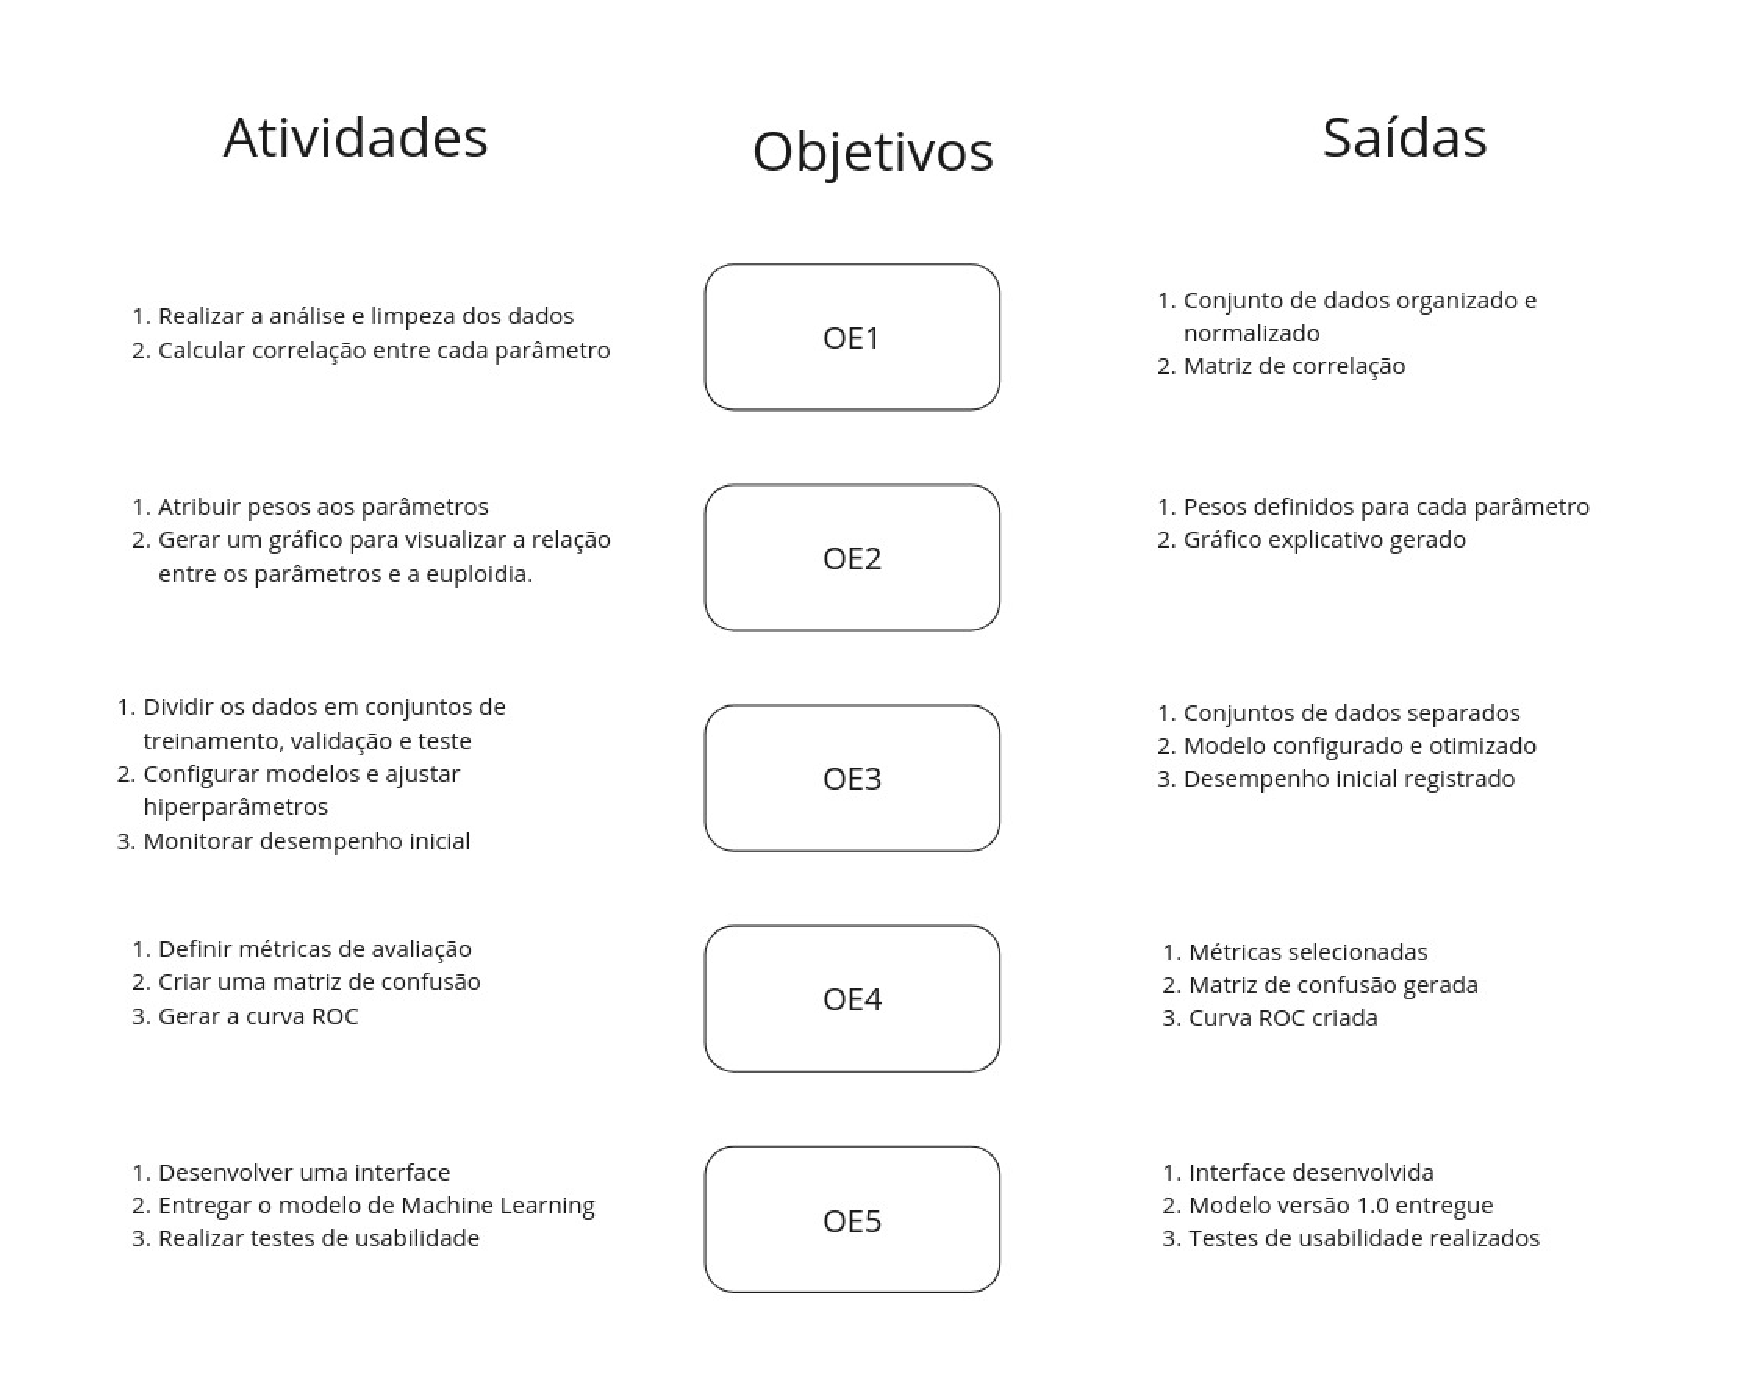
\includepdf[pages=-, scale=1, pagecommand={}, fitpaper=true]{figuras/fluxoatividades.pdf}

\section{Composição e estrutura do trabalho}
Este trabalho foi organizado da seguinte maneira:

\textbf{Capítulo 2}: intitulado "Referencial Teórico", foi abordado os principais conceitos que apoiam a contextualização deste trabalho;

\textbf{Capítulo 3}: intitulado "Metodologia", detalhou seção 1.5. Será descrito os procedimentos e métodos utilizados na pesquisa indicando um planejamento de trabalho, as atividades realizadas e os resultados esperados;

\textbf{Capítulo 4}: intitulado "Planejamento", apresenta a previsão de término de cada atividade e fase propostas;

\textbf{Capítulo 5}: intitulado "Execução e Resultados Preliminares", apresenta o que foi concluído durante o período de escrita deste TCC;

\textbf{Capítulo 6}: intitulado "Considerações e Trabalhos Futuros", foi retomada todas as atividades e produtos obtidos até o momento da escrita do capítulo.